% Options for packages loaded elsewhere
\PassOptionsToPackage{unicode}{hyperref}
\PassOptionsToPackage{hyphens}{url}
%
\documentclass[
]{article}
\usepackage{amsmath,amssymb}
\usepackage{lmodern}
\usepackage{iftex}
\ifPDFTeX
  \usepackage[T1]{fontenc}
  \usepackage[utf8]{inputenc}
  \usepackage{textcomp} % provide euro and other symbols
\else % if luatex or xetex
  \usepackage{unicode-math}
  \defaultfontfeatures{Scale=MatchLowercase}
  \defaultfontfeatures[\rmfamily]{Ligatures=TeX,Scale=1}
\fi
% Use upquote if available, for straight quotes in verbatim environments
\IfFileExists{upquote.sty}{\usepackage{upquote}}{}
\IfFileExists{microtype.sty}{% use microtype if available
  \usepackage[]{microtype}
  \UseMicrotypeSet[protrusion]{basicmath} % disable protrusion for tt fonts
}{}
\makeatletter
\@ifundefined{KOMAClassName}{% if non-KOMA class
  \IfFileExists{parskip.sty}{%
    \usepackage{parskip}
  }{% else
    \setlength{\parindent}{0pt}
    \setlength{\parskip}{6pt plus 2pt minus 1pt}}
}{% if KOMA class
  \KOMAoptions{parskip=half}}
\makeatother
\usepackage{xcolor}
\usepackage[margin = 0.6in]{geometry}
\usepackage{longtable,booktabs,array}
\usepackage{calc} % for calculating minipage widths
% Correct order of tables after \paragraph or \subparagraph
\usepackage{etoolbox}
\makeatletter
\patchcmd\longtable{\par}{\if@noskipsec\mbox{}\fi\par}{}{}
\makeatother
% Allow footnotes in longtable head/foot
\IfFileExists{footnotehyper.sty}{\usepackage{footnotehyper}}{\usepackage{footnote}}
\makesavenoteenv{longtable}
\usepackage{graphicx}
\makeatletter
\def\maxwidth{\ifdim\Gin@nat@width>\linewidth\linewidth\else\Gin@nat@width\fi}
\def\maxheight{\ifdim\Gin@nat@height>\textheight\textheight\else\Gin@nat@height\fi}
\makeatother
% Scale images if necessary, so that they will not overflow the page
% margins by default, and it is still possible to overwrite the defaults
% using explicit options in \includegraphics[width, height, ...]{}
\setkeys{Gin}{width=\maxwidth,height=\maxheight,keepaspectratio}
% Set default figure placement to htbp
\makeatletter
\def\fps@figure{htbp}
\makeatother
\setlength{\emergencystretch}{3em} % prevent overfull lines
\providecommand{\tightlist}{%
  \setlength{\itemsep}{0pt}\setlength{\parskip}{0pt}}
\setcounter{secnumdepth}{5}
\usepackage{wrapfig} \usepackage{float} \usepackage{dcolumn} \usepackage{amsmath} \usepackage{array} \usepackage{amsfonts} \floatplacement{figure}{H}
\usepackage{subfig}
\ifLuaTeX
  \usepackage{selnolig}  % disable illegal ligatures
\fi
\IfFileExists{bookmark.sty}{\usepackage{bookmark}}{\usepackage{hyperref}}
\IfFileExists{xurl.sty}{\usepackage{xurl}}{} % add URL line breaks if available
\urlstyle{same} % disable monospaced font for URLs
\hypersetup{
  pdftitle={Predicting Customer Approval of Motorcycles},
  pdfauthor={Amina Alavi, Gary Kong, Vernon Robinson, Elizabeth Willard},
  hidelinks,
  pdfcreator={LaTeX via pandoc}}

\title{Predicting Customer Approval of Motorcycles}
\usepackage{etoolbox}
\makeatletter
\providecommand{\subtitle}[1]{% add subtitle to \maketitle
  \apptocmd{\@title}{\par {\large #1 \par}}{}{}
}
\makeatother
\subtitle{W203 Lab 2 Report}
\author{Amina Alavi, Gary Kong, Vernon Robinson, Elizabeth Willard}
\date{}

\begin{document}
\maketitle

{
\setcounter{tocdepth}{2}
\tableofcontents
}
\newpage
\setcounter{page}{1}

\hypertarget{introduction}{%
\section{Introduction}\label{introduction}}

Motorcycle manufacturers face several key challenges in the current
global motorcycle market. The market is highly competitive, with
368 distinct brands and 7677
models in bikez.com's 2013 - 22 database of motorcycles. Meanwhile, easy
access to information makes customers more discriminating in purchasing
decisions. Therefore, there is a need to design products in a
data-driven way to satisfy customer preferences.

Many different aspects of product design could impact how well a
motorcycle is received by customers. These include, but are not limited
to, motorcycle category, engine responsiveness, transmission, handling,
suspension, and styling. Nonetheless, engine responsiveness is one of
the most important features customers look for. This analysis provides a
starting point toward understanding how engine responsiveness impacts
customer acceptance by asking the following research question:

\begin{quote}
  \textit{How does motorcycle engine responsiveness impact customer approval?}
\end{quote}

The answer to this question could help quantify how engine
responsiveness impacts customer approval, especially compared to other
features. Insights from our analysis are particularly relevant to
product design teams, who can use this information to focus on designing
products with features more likely to satisfy customer preferences.
Investors may also use the outcomes of this research to better predict a
given motorcycle's success.

\hypertarget{data-and-methodology}{%
\section{Data and Methodology}\label{data-and-methodology}}

The data in this study came from bikez.com, which provides high-quality
motorcycle specification data from 1894 to 2022. A custom scraper
extracted the data on 30 April 2022 to enrich an existing used
motorcycle dataset for a Kaggle hackathon competition. It was compiled
and made publicly available by Emmanuel F. Werr. The observational data
includes 28 unique features that describe a given motorcycle. The data
source is a .CSV file containing information of 38,472 motorcycles, each
row representing a motorcycle (based on brand, model, and year
combination).

To operationalize our Y concept of customer approval, we used the
\emph{rating} variable, a mean of customer review scores (1-5 scale). Rating
is a strong proxy for customer approval as it directly quantifies how
well-received a motorcycle is by customers. Customers' individual
ratings are ordinal but can be treated as interval due to equal
differences between categories. Also, the rating variable in the dataset
is metric as it is an aggregated mean of individual ratings.

To operationalize our X concept of engine responsiveness, we used the
\emph{torque} variable, which captures maximum torque in Newton-meters (Nm).
The higher the torque, the faster the bike accelerates. Torque is one of
the most important parameters that determine the responsiveness of a
motorbike. We included \emph{category}, \emph{wheelbase}, \emph{cooling system}, \emph{front
brakes}, \emph{transmission type}, and \emph{year} as secondary X variables.

The raw dataset includes 38472 motorcycles. We limited the
dataset to motorcycles with a \emph{year} between 2013 - 22, which leaves
14422 observations. We removed observations with missing
values for any of our operationalization variables. First, we removed
motorcycles with missing \emph{rating} values, which leaves
1327 observations. No motorcycles had missing values for
\emph{torque}, \emph{fuel capacity} and \emph{wheelbase}. Second, we removed
motorcycles with missing \emph{cooling system} values, which leaves
1325 observations. Third, we removed motorcycles
with missing \emph{front brake} values, which leaves
1324 observations. Fourth, we removed motorcycles
with missing \emph{transmission type} values, which leaves
1296 observations.

We also manipulated four categorical variables (\emph{cooling system}, \emph{front
brakes}, \emph{transmission type}, and \emph{category}), reducing the number of
categories in each to simplify the model and facilitate model
interpretation. For \emph{cooling system}, we grouped similar categories
(i.e., ``Air'' and ``Oil \& Air'') together. For \emph{front brakes},
\emph{transmission type}, and \emph{category}, we removed observations belonging
to categories with a small number of Ns, which leaves
1135 observations.

To choose X variables to include in our model, we initially conducted a
correlation analysis of all continuous variables (see Figure
\ref{fig:side-by-side-plots}a). As the sample size after wrangling
(n=1135) is not very large, we decided to not divide
our data into exploratory and confirmation sets. We chose \emph{torque} over
\emph{power} as the two are highly correlated (see Figure
\ref{fig:side-by-side-plots}a), since power is a function of torque and
speed (RPM). Some variables (\emph{bore, stroke}, \emph{displacement}) had been
excluded from our research at the outset due to concerns of correlation
to \emph{power} and \emph{torque,} which is confirmed here. Excluding these highly
correlated variables minimizes the risk of having outcome variables on
the right-hand side. While we initially hypothesized that \emph{seat height}
could be an explanatory variable, we chose to omit it as there is no
correlation between \emph{seat height} and \emph{rating}. Also, since \emph{wheelbase}
and \emph{dry weight} are highly correlated, we dropped \emph{dry weight} and kept
\emph{wheelbase}, which is itself less correlated to \emph{torque}.

\begin{figure}
\subfloat[Correlations\label{fig:side-by-side-plots-1}]{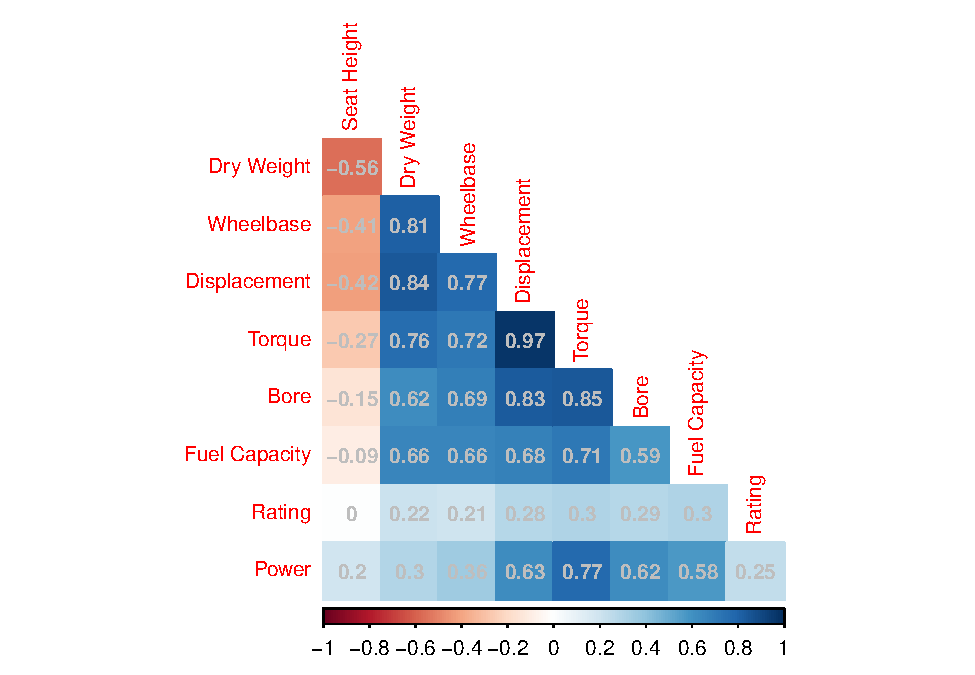
\includegraphics[width=0.5\linewidth]{W203_Project2_Predicting-Customer-Approval-of-Motorcycles_files/figure-latex/side-by-side-plots-1} }\subfloat[Pairwise Plots\label{fig:side-by-side-plots-2}]{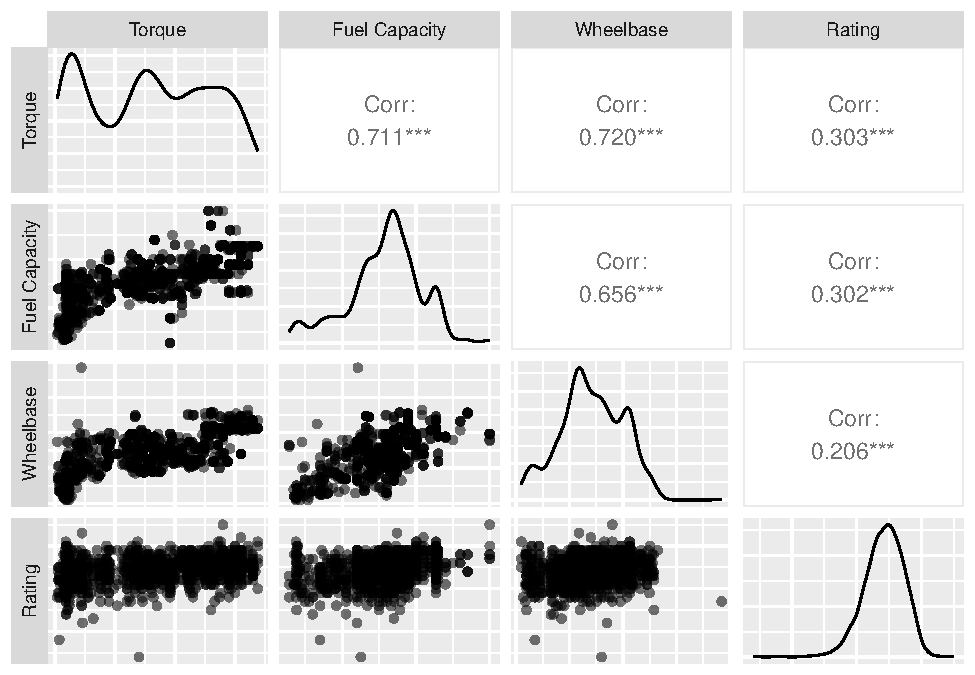
\includegraphics[width=0.5\linewidth]{W203_Project2_Predicting-Customer-Approval-of-Motorcycles_files/figure-latex/side-by-side-plots-2} }\caption{Pearson Correlation of Continuous X Variables and Pairwise Plots of Continuous X and Y Variables}\label{fig:side-by-side-plots}
\end{figure}

The bottom three plots in Figure \ref{fig:side-by-side-plots}b show
\emph{rating} as a function of \emph{torque}, \emph{fuel capacity}, and \emph{wheelbase}.
Notably, \emph{rating} appears to increase as \emph{torque} and \emph{fuel capacity}
increase, with moderate correlations between \emph{fuel capacity} and
\emph{rating}, and \emph{torque} and \emph{rating}. In contrast, the relationship
between \emph{wheelbase} and \emph{rating} appears less strong but is still
significant. We chose to still include \emph{wheelbase} as an X variable /
covariate to reduce omitted variable bias.

Several categorical X variables were intentionally excluded from our
analysis to minimize complexity. \emph{Fuel system}, \emph{fuel control}, \emph{front
suspension}, \emph{rear suspension}, \emph{color options} had excessively large
numbers of distinct categories, making them unsuitable for regression.
\emph{Rear brakes} was excluded as \emph{front brakes} are considered more
important. \emph{Engine cylinder}, \emph{engine stroke} and \emph{gearbox} were
excluded as categories were ordinal and correlated with \emph{torque}, so
inclusion would have led to outcome variables on right-hand side. Based
on the above, we specified five models:

\textbf{Model 1:} We wanted our first model to be simple and thus only used
our primary X variable, \emph{torque}, to predict \emph{rating}, as exploratory
plots show a linear relationship between the two variables. In this
model, \(\beta_1\) represents the change in \emph{rating} for each unit
increase in \emph{torque} (all else kept constant). The model is:

\[
  \widehat{Rating}=\beta_0 + \beta_1\cdot Torque + \epsilon
\] \textbf{Model 2:} We included all shortlisted X variables to assess
statistical significance and to minimize omitted variable bias. All
\(\beta\)s (except \(\beta_0\)) represent change in \emph{rating} for each unit
change of the X variable (all else kept constant). The model is:

\begin{equation}
  \begin{aligned}
      \widehat{Rating}=\beta_0 + \beta_1\cdot Torque +
             \beta_2\cdot Fuel Capacity +
               \beta_3\cdot Wheelbase + \\
                 \beta_4\cdot Cooling System +
                  \beta_5\cdot Front Breaks +
                   \beta_6\cdot Transmission Type
                      + \epsilon
  \end{aligned}
\end{equation}

\textbf{Model 3:} Initial data exploration suggested that \emph{category} affects
\emph{rating}. Thus, we included \emph{category} to improve model fit\footnote{The categories are represented by i in the equation. Indicator
  variables are ``Classic'', ``Custom cruiser'', ``Enduro / offroad'',
  ``Naked bike'', ``Scooter'', ``Sport'', ``Super motard'', ``Touring''. The
  baseline category is ``All round''.}. Also,
to simplify the model, we grouped all X variables with little
significance under \(\mathbf{Z}\boldsymbol{\gamma}\). \(\mathbf{Z}\) is a
row vector for the covariates and \(\boldsymbol{\gamma}\) is a column
vector of coefficients.

\begin{equation}
  \begin{aligned}
  \widehat{Rating}=\beta_0 + \beta_1\cdot Torque +
           \beta_2\cdot Fuel Capacity +
                  \beta_i\cdot Category_{i} +
                   \mathbf{Z}\boldsymbol{\gamma}
                    + \epsilon
  \end{aligned}
\end{equation}

\textbf{Model 4:} The mean of \emph{rating} appears to vary by year. We thus added
\emph{year} to our fourth model to correct for this and to improve the
model's accuracy. \emph{Year} is included as part of
\(\mathbf{Z}\boldsymbol{\gamma}\) given many categories.

\textbf{Model 5:} For our final model we added \emph{brand}. Like \emph{year}, the mean
of \emph{rating} from brand to brand varies significantly. We added \emph{brand}
to our fifth model based on the same rationale as adding \emph{year,}
including \emph{brand} as part of \(\mathbf{Z}\boldsymbol{\gamma}\).

We considered modeling interactions between \emph{category} and other
variables. However, the large number of categories would lead to
excessive complexity in the model for the purposes of this assignment.

\hypertarget{results}{%
\section{Results}\label{results}}

\begin{table}[H] \centering 
  \caption{Estimated Regressions} 
  \label{} 
\small 
\begin{tabular}{@{\extracolsep{-1.5pt}}lD{.}{.}{-3} D{.}{.}{-3} D{.}{.}{-3} D{.}{.}{-3} D{.}{.}{-3} } 
\\[-1.8ex]\hline 
\hline \\[-1.8ex] 
 & \multicolumn{5}{c}{Output Variable: Mean Rating (1-5 scale)} \\ 
\cline{2-6} 
\\[-1.8ex] & \multicolumn{5}{c}{Rating} \\ 
\\[-1.8ex] & \multicolumn{1}{c}{(1)} & \multicolumn{1}{c}{(2)} & \multicolumn{1}{c}{(3)} & \multicolumn{1}{c}{(4)} & \multicolumn{1}{c}{(5)}\\ 
\hline \\[-1.8ex] 
 Torque (Nm) & 0.002^{***} & 0.002^{***} & 0.002^{***} & 0.002^{***} & 0.001^{*} \\ 
  & (0.0002) & (0.0003) & (0.0004) & (0.0004) & (0.0005) \\ 
  & & & & & \\ 
 Fuel Capacity (Litres) &  & 0.013^{***} & 0.016^{***} & 0.016^{***} & 0.018^{***} \\ 
  &  & (0.003) & (0.003) & (0.003) & (0.004) \\ 
  & & & & & \\ 
 Category: Classic &  &  & 0.068 & 0.063 & 0.016 \\ 
  &  &  & (0.050) & (0.050) & (0.053) \\ 
  & & & & & \\ 
 Category: Custom / cruiser &  &  & -0.183^{**} & -0.174^{**} & -0.161^{*} \\ 
  &  &  & (0.065) & (0.064) & (0.067) \\ 
  & & & & & \\ 
 Category: Enduro / offroad &  &  & -0.148^{***} & -0.139^{**} & -0.198^{***} \\ 
  &  &  & (0.044) & (0.045) & (0.048) \\ 
  & & & & & \\ 
 Category: Naked bike &  &  & -0.105^{**} & -0.095^{**} & -0.109^{**} \\ 
  &  &  & (0.035) & (0.035) & (0.038) \\ 
  & & & & & \\ 
 Category: Scooter &  &  & -0.028 & -0.014 & -0.094 \\ 
  &  &  & (0.062) & (0.061) & (0.081) \\ 
  & & & & & \\ 
 Category: Sport &  &  & -0.174^{***} & -0.159^{***} & -0.187^{***} \\ 
  &  &  & (0.039) & (0.040) & (0.043) \\ 
  & & & & & \\ 
 Category: Super motard &  &  & -0.080^{*} & -0.069 & -0.134^{**} \\ 
  &  &  & (0.040) & (0.041) & (0.044) \\ 
  & & & & & \\ 
 Category: Touring &  &  & -0.127^{*} & -0.117 & -0.087 \\ 
  &  &  & (0.062) & (0.062) & (0.063) \\ 
  & & & & & \\ 
 Constant & 3.274^{***} & 3.420^{***} & 3.471^{***} & 3.449^{***} & 3.680^{***} \\ 
  & (0.019) & (0.196) & (0.229) & (0.231) & (0.277) \\ 
  & & & & & \\ 
\hline \\[-1.8ex] 
Wheelbase (mm) &  & \checkmark & \checkmark & \checkmark  & \checkmark \\ 
Cooling System &  & \checkmark & \checkmark & \checkmark & \checkmark \\ 
Front Brakes &  & \checkmark & \checkmark & \checkmark & \checkmark \\ 
Transmission Type &  & \checkmark & \checkmark & \checkmark & \checkmark \\ 
Year &  &  &  & \checkmark & \checkmark \\ 
Brand &  &  &  &  & \checkmark \\ 
\hline &  &  &  &  &  \\ 
Observations & \multicolumn{1}{c}{1,135} & \multicolumn{1}{c}{1,135} & \multicolumn{1}{c}{1,135} & \multicolumn{1}{c}{1,135} & \multicolumn{1}{c}{1,135} \\ 
R$^{2}$ & \multicolumn{1}{c}{0.092} & \multicolumn{1}{c}{0.114} & \multicolumn{1}{c}{0.161} & \multicolumn{1}{c}{0.167} & \multicolumn{1}{c}{0.260} \\ 
Residual Std. Error & \multicolumn{1}{c}{0.296 (df = 1133)} & \multicolumn{1}{c}{0.293 (df = 1128)} & \multicolumn{1}{c}{0.286 (df = 1120)} & \multicolumn{1}{c}{0.286 (df = 1111)} & \multicolumn{1}{c}{0.276 (df = 1059)} \\ 
\hline 
\hline \\[-1.8ex] 
Significance levels & \multicolumn{5}{r}{$^{*}$p$<$0.05; $^{**}$p$<$0.01; $^{***}$p$<$0.001} \\ 
\end{tabular} 
\end{table}

Table 1 shows the results of five representative regressions\footnote{In model 2, wheelbase, cooling system, brakes, transmission type
  were part of the main model. However, they were pushed down as
  covariates starting from model 3 as they were not statistically
  significant. Robust standard errors are shown in parentheses.}. The
R-squared values increase as we go across the models, which indicates
that the models become increasingly predictive. Across all models, the
estimated coefficient for our primary X variable, \emph{torque}, was highly
statistically significant. Point estimates were consistent for the first
four models at 0.002, and was
0.001 for model 5. To provide a
sense of scale, consider a manufacturer which increased the torque of a
motorcycle by 300 Nm, all else being equal. Applying model 5, the
motorcycle's rating is expected to increase by
0.38.

Across all models, the coefficient for \emph{fuel capacity} was also highly
statistically significant. Point estimates ranged from
0.01
to
0.018.
Another example to consider is two motorcycles with fuel capacity
differing by 12 liters, all else being the same. Applying model 5, the
rating of the motorcycle with the higher fuel capacity is expected to
exceed the motorcycle with the lower fuel capacity by
0.21.

Most coefficients for \emph{category} indicators were statistically
significant. An example to consider is the ``Enduro / offroad'' category.
Applying model 5, a motorcycle in the ``Enduro / offroad'' category is
expected to have
-0.2 lower ratings
than the baseline category (``All round'').

As previously noted, other covariates were included to adjust for
omitted variable bias. Notably, the coefficients for \emph{wheelbase},
\emph{cooling system}, \emph{front brakes}, \emph{transmission type} were not
statistically significant, as such, estimated coefficients for these
should not be strictly used to make design decisions if the goal is to
increase customer approval. We also note that \emph{year} and \emph{brand}, while
being statistically significant for particular categories, are not
practically significant as these are not parameters that a manufacturer
can affect.

From a motorcycle manufacturer's point of view, when deciding which
specifications to focus on, \emph{torque} and \emph{fuel capacity} seem to affect
customer approval the most. Since \emph{torque} is highly correlated with
\emph{power}, \emph{bore}, \emph{stroke} and displacement, these should also be
included in the list of specifications to be optimized for if the goal
is higher customer ratings. Manufacturers should also look into focusing
on ``Classic'' motorbikes as this category is most likely to lead to the
highest customer ratings.

\hypertarget{limitations}{%
\section{Limitations}\label{limitations}}

Consistent regression estimates require an assumption of independent and
identically distributed (iid) observations. Motorcycles in the dataset
belong to various brands, and motorcycles from specific brands may share
common characteristics, so observations may not be fully independent. We
partially account for this possibility in the fifth model by including
\emph{brand} as a covariate. Furthermore, observations may not be strictly
identically distributed as motorcycles in the dataset were drawn from
different years. We partially account for this possibility by
restricting the \emph{year} to 2013 - 22, and by including \emph{year} as a
covariate in models four and five.

Consistent regression estimates also require that a unique best linear
predictor describes the population distribution. As shown in Figure
\ref{fig:side-by-side-plots}b, there is no visual evidence of
heavy-tailed distributions. There is also no perfect collinearity as
correlations between pairs of X variables are all less than one, and no
variables were dropped when fitting the regressions.

Heteroskedastic error is apparent in Figure
\ref{fig:side-by-side-plots}b. This is less of a concern for the Large
Sample Models used but is nonetheless accounted for by using robust
standard errors. Additionally, it is unclear whether bikez.com used
random sampling in choosing which motorcycles to include in its
database. As such, there may be limitations as to the generalizeability
of our findings across all motorcycles. Finally, while our models
identified linear relationships between \emph{rating}. and \emph{torque} and \emph{fuel
capacity}, these relationships may not necessarily hold for very high
values of \emph{torque} and \emph{fuel capacity}, particularly as \emph{rating} should
have a maximal value of 5.

Regarding structural limitations, a potential source of omitted variable
bias is fuel efficiency, which did not have a corresponding variable in
our data source. We postulate that \emph{torque} has a negative relationship
with \emph{fuel efficiency}, and that \emph{fuel efficiency} has a positive
relationship with \emph{rating}. As such, the direction of bias would be
negative and towards zero, implying that the true effect of \emph{torque} on
\emph{rating} is larger than the estimated effect. We do not consider reverse
causality present, as rating should not cause changes in our X
variables. We also do not have outcome variables on the right-hand side
as X variable selection accounted for this (e.g., choosing torque over
power due to correlation).

\hypertarget{conclusion}{%
\section{Conclusion}\label{conclusion}}

This study estimated the relationship between key motorcycle features
and customer approval of a motorcycle, proxied by mean ratings. We also
described and measured how motorcycle category predicts ratings.
Follow-up models could include interactions between motorcycle
categories and design features such as torque and fuel capacity, as the
impact of different motorcycle features on ratings could differ
depending on the motorcycle category. Follow-up models could also use
simplified versions of categorical variables which were excluded due to
excessive distinct categories. Motorcycle manufacturers may want to
know, for example, whether there are benefits to choosing specific types
of tires or suspension systems. Future research could also incorporate
other datasets (e.g., sales data) to provide a more holistic view of
product success. The ultimate goal of this line of work is to provide
accurate tools for motorcycle manufacturers to develop motorcycles that
are more likely to achieve success and reduce uncertainty in the design
process.

\end{document}
